\documentclass[tikz,convert={outext=.svg,command=\unexpanded{{pdf2svg \infile\space \outfile}}}]{standalone}

\usetikzlibrary{automata,positioning,arrows.meta,shapes,shapes.geometric}

\tikzset{
%-{Stealth[length=3mm,width=2mm]}, % makes the edges directed
>={Stealth[length=3mm,width=2mm]}, % makes the arrow heads bold
node distance=3cm, % specifies the minimum distance between two nodes. Change if necessary.
every state/.style={ultra thick},
every path/.style={color=white,thick},
every node/.style={font=\Large,align=center},
initial text=$ $,
on grid,
auto
}

\newcommand\hred[1]{\textbf{\textcolor{red!50!white}{#1}}}
\newcommand\hgreen[1]{\textbf{\textcolor{green!50!white}{#1}}}
\newcommand\hyellow[1]{\textbf{\textcolor{yellow!50!white}{#1}}}
\newcommand\hwhite[1]{\textbf{\textcolor{white}{#1}}}

\newcommand\rd[1]{\textcolor{red!50!white}{#1=R}}
\newcommand\g[1]{\textcolor{green!50!white}{#1=G}}
\newcommand\y[1]{\textcolor{yellow!50!white}{#1=Y}}
\newcommand\w[1]{\textcolor{white}{#1}}

\begin{document}
\bf
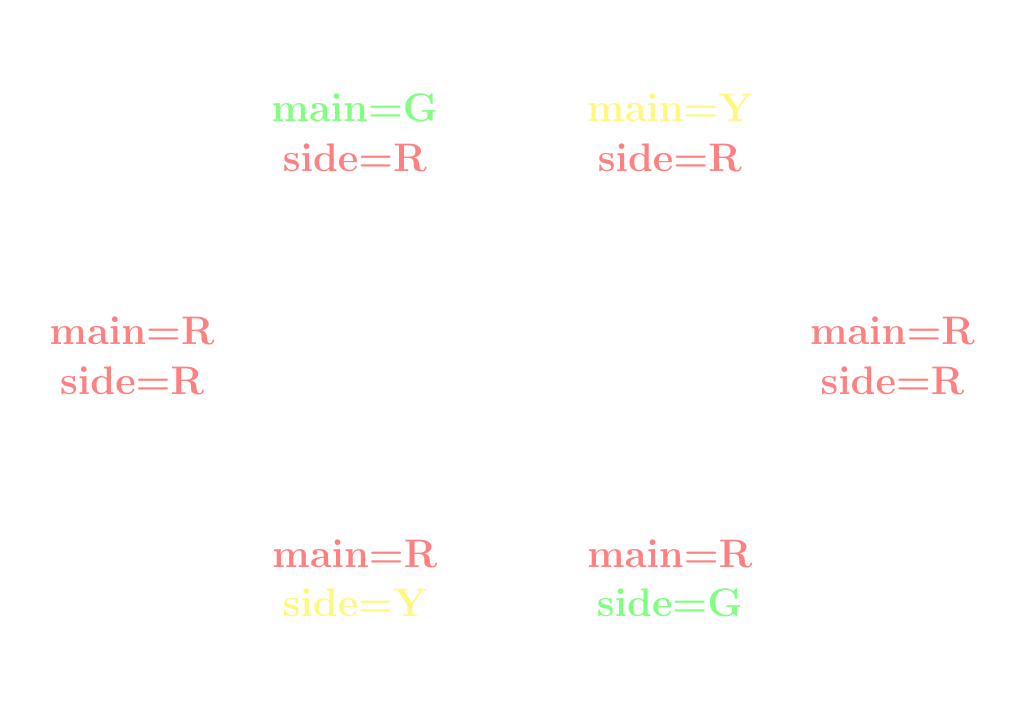
\begin{tikzpicture}[state/.style={circle, draw, minimum size=1.5cm, node distance=4cm}]
   \node[state] (rr1) {\hred{main=R} \\ \hred{side=R}};
   \node[state, text=white] (gr)  [above right=of rr1] {\hgreen{main=G} \\ \hred{side=R}};
   \node[state] (yr)  [right=of gr] {\hyellow{main=Y} \\ \hred{side=R}};
   \node[state] (rr2) [below right=of yr] {\hred{main=R} \\ \hred{side=R}};
   \node[state] (rg)  [below left=of rr2] {\hred{main=R} \\ \hgreen{side=G}};
   \node[state] (ry)  [left=of rg] {\hred{main=R} \\ \hyellow{side=Y}};
   \path[->]
    (rr1) edge (gr)
    (gr)  edge (yr)
    (yr)  edge (rr2)
    (rr2) edge (rg)
    (rg)  edge (ry)
    (ry)  edge (rr1);
\end{tikzpicture}
\end{document}
